\documentclass[aspectratio=1610]{beamer}

\usepackage[utf8]{inputenc}
\usepackage{graphicx}
\usepackage{amssymb}
\usepackage[export]{adjustbox}
\usetheme{Frankfurt}
\usefonttheme[onlymath]{serif}
\usepackage[super]{nth}
\graphicspath{{./Figures/}}
\usepackage{hyperref}
\hypersetup{
    colorlinks=true,
    linkcolor=athgold,
    filecolor=magenta,      
    urlcolor=cyan,
}
\usepackage{wasysym}
\definecolor{satinsheengold}{rgb}{.7608 .5569 0.0471}
\definecolor{athgold}{rgb}{0.8078, 0.7216, 0.5333}
\definecolor{dkgray}{rgb}{.2157, .2275, .2118}
\setbeamercolor{structure}{fg=satinsheengold}
\setbeamercolor{title}{fg=black}
\setbeamercolor{title in head/foot}{fg=black, bg=satinsheengold}
\setbeamercolor{author}{fg=dkgray}
\setbeamercolor{frametitle}{fg=black}
\setbeamercolor{author in head/foot}{fg=black, bg=satinsheengold}
\setbeamercolor{institute in head/foot}{bg=satinsheengold}
\setbeamercolor{date in head/foot}{bg=satinsheengold}
\setbeamercolor{section in foot}{fg=white, bg=dkgray}
\setbeamercolor{section in head}{fg = athgold, bg = black} 
\setbeamercolor{navigation symbols}{fg=gray}
\setbeamercolor{block title}{bg=athgold, fg = black}
\setbeamercolor{item projected}{fg=black}
\setbeamercolor{footlinecolor}{fg = black, bg = white}
\setbeamertemplate{blocks}[rounded][shadow=false]
\setbeamertemplate{enumerate items}[circle]
%\setbeamertemplate{footline}[frame number]
%Adding frame #s
\setbeamertemplate{navigation symbols}{%
    \usebeamerfont{footline}%
    \usebeamercolor[bg]{footline}%
    \hspace{1em}%
    %\insertframenumber/\inserttotalframenumber
}
\setbeamertemplate{footline}[text line]{%
  \begin{beamercolorbox}[wd=\paperwidth,ht=2.25ex,dp=1ex]{section in head}%
	\hspace{.5em} 	
 	\makebox[0pt][l]{\,\color{athgold}{\insertsection}}
 	 \hspace*{\fill}\insertshortauthor\hspace*{\fill}%
 	 \llap{\insertpagenumber\,/\,\insertpresentationendpage\,}	
 	 \hspace{.5em}
  \end{beamercolorbox}
}

\setbeamertemplate{headline}[text line]{%
  \begin{beamercolorbox}[wd=\paperwidth,ht=2.25ex,dp=1ex,center]{section in head}%
 BME 695 $|$ Numerical Methods
 %\inserttitle
  \end{beamercolorbox}
}


\title{Coding Assignment 2}
\author[Andrew Sivaprakasam]{Andrew Sivaprakasam}

\date{04/18/2021}

%Change this to section titles when you have a pres with multiple sections
\section{\insertshorttitle}
\begin{document}

\frame{\titlepage}

\section{Problem 1}

\begin{frame}[fragile]
\frametitle{Problem 1 | Cubic Spline Implementation}

After implementing the spline equations, and solving the system of equations for the natural/free spline, complete spline, parabolically terminated, and not-a-knot end conditions, I generated these plots. The different end conditions are a parameter in my \verb|spline_2()| function.

\centering
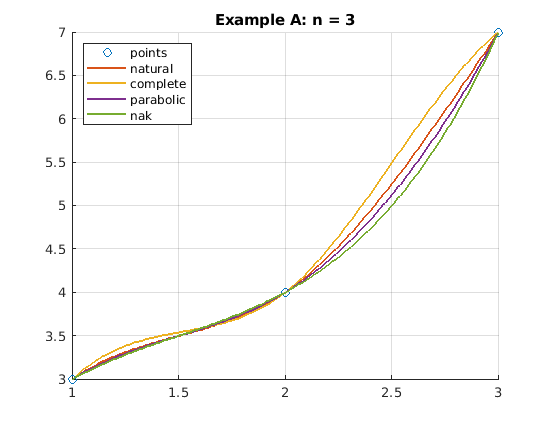
\includegraphics[width = .49\textwidth]{1a}
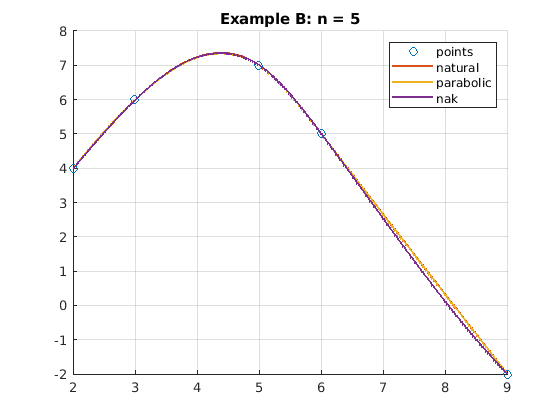
\includegraphics[width = .49\textwidth]{1b}
\end{frame}

\begin{frame}
\frametitle{Problem 1 | Cubic Spline Implementation}
I also checked this implementation using the Runge function $\frac{1}{1+25x^2}$ :

\centering 
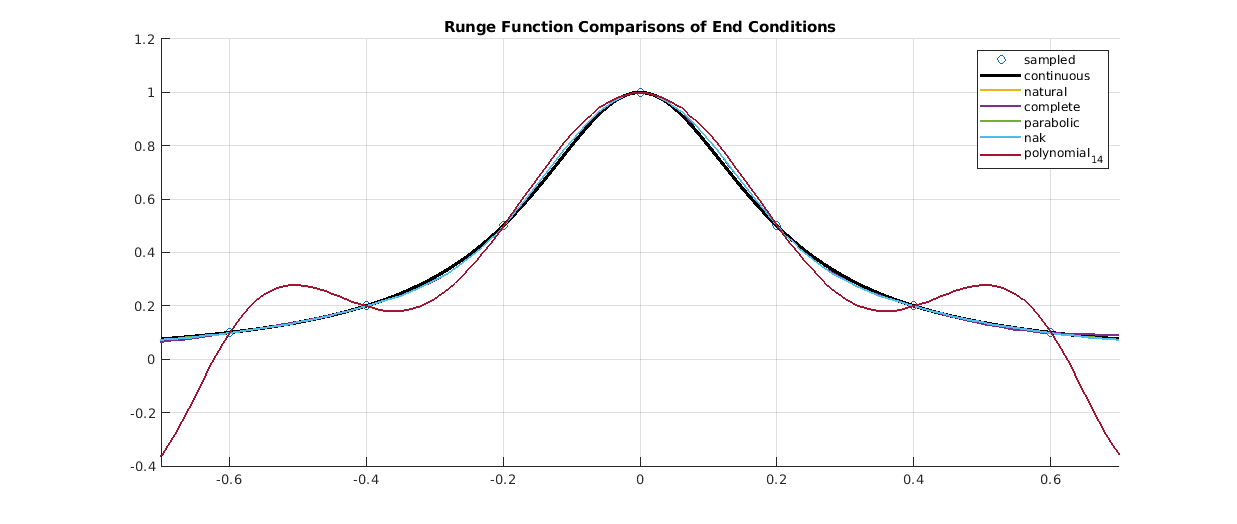
\includegraphics[width = .95\textwidth]{1c}
\textit{Note how the high-order polynomial fit is unstable/oscillatory at the ends, while the spline interpolations handle this problem nicely.}
\end{frame}

\section{Problem 2}

\begin{frame}
\frametitle{Problem 2 $|$ Task 1 | Plotting }

Here are my 2D \& 3D contour maps for the:

\begin{columns}
\begin{column}{.5\textwidth}

\vspace{1em}
\centering
\textbf{Beale Function:}

\scalebox{.7}{$f(x,y) = (1.5-x + xy) + (2.25 - x + xy^3)^2 + (2.625 - x + xy)^2$ 
}
\vspace{.5em}
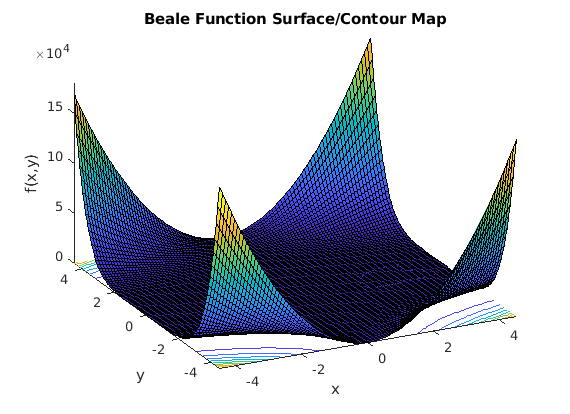
\includegraphics[width = .95\textwidth]{2_beals}
\end{column}
\begin{column}{.5\textwidth}

\vspace{1.5em}
\centering
\textbf{Rosenbrock Function ($n = 2$):}

\scalebox{.7}{$f(x) = \sum^{n-1} _{i=1}[100(x_{i+1}-x_{i})^2]$ 
}
\vspace{.5em}
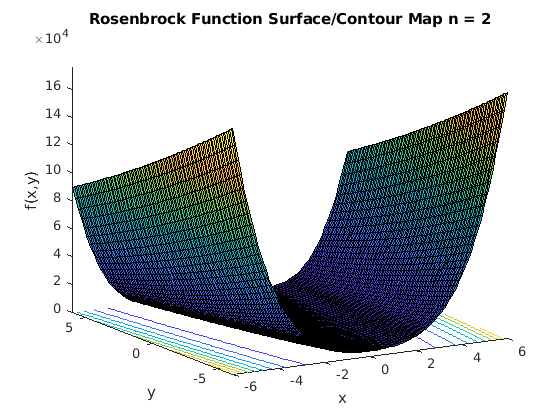
\includegraphics[width = .95\textwidth]{2_rbrocks}
\end{column}
\end{columns}
\end{frame}

\begin{frame}[fragile]
\frametitle{Problem 2 $|$ Task 2a/b | Nelder-Mead Optimization}

\textbf{Please see code} \verb|p2.m|. The Beale function was minimized successfully to $(3.0, 0.5)$ where $f(x,y) = 0$, as long as the starting point was $(4.5 , 4.5)$ instead of  $(-4.5 , -4.5)$.

The Rosenbrock function was minimize to $(1,1,1,1)$ with the starting point being (2,2,2,2). 
 
\end{frame}

\begin{frame}[fragile]
\frametitle{Problem 2 $|$ Task 3}

\small{I had some issues with my implementation of Response Surface optimization of these two functions. Since we were asked to continuously fit a quadratic instead of a linear function \textit{then} a quadratic, the minimization may have chosen points past the minimum, resulting in oscillations about the true minimum. Here are plots of where my minimum points (blue) ended up settling relative to these surfaces.}

\vspace{1em}
\centering
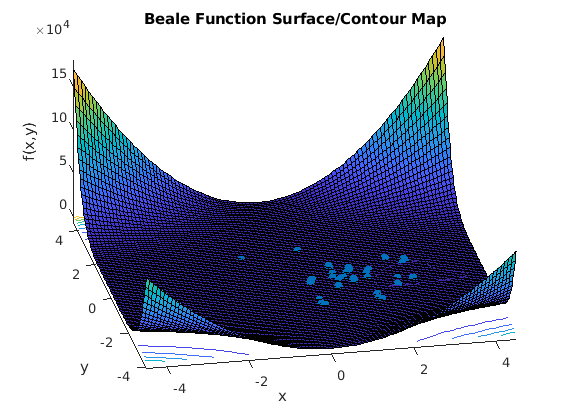
\includegraphics[width = .49\textwidth]{2_beale_rsm}
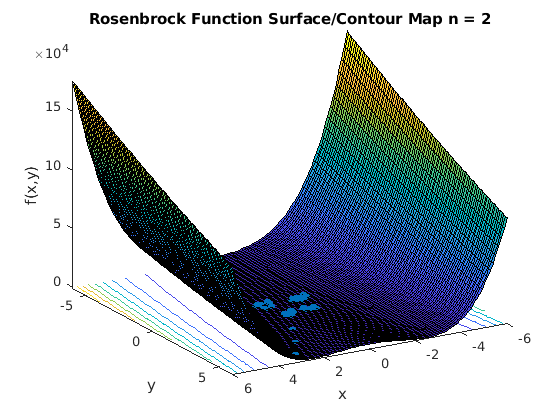
\includegraphics[width = .49\textwidth]{2_rbrock_rsm}
\end{frame}

\section{Problem 3}
\begin{frame}
\frametitle{Problem 3}

Here are the simulations I ran of the state-transition model. I ran 1000x1000 LHS design instead of 500, in order to better estimate a ground truth/better train my models. The data may be visualized as either a 2D or 3D plot, but I think the 3D one is prettier.

\vspace{1em}
\centering
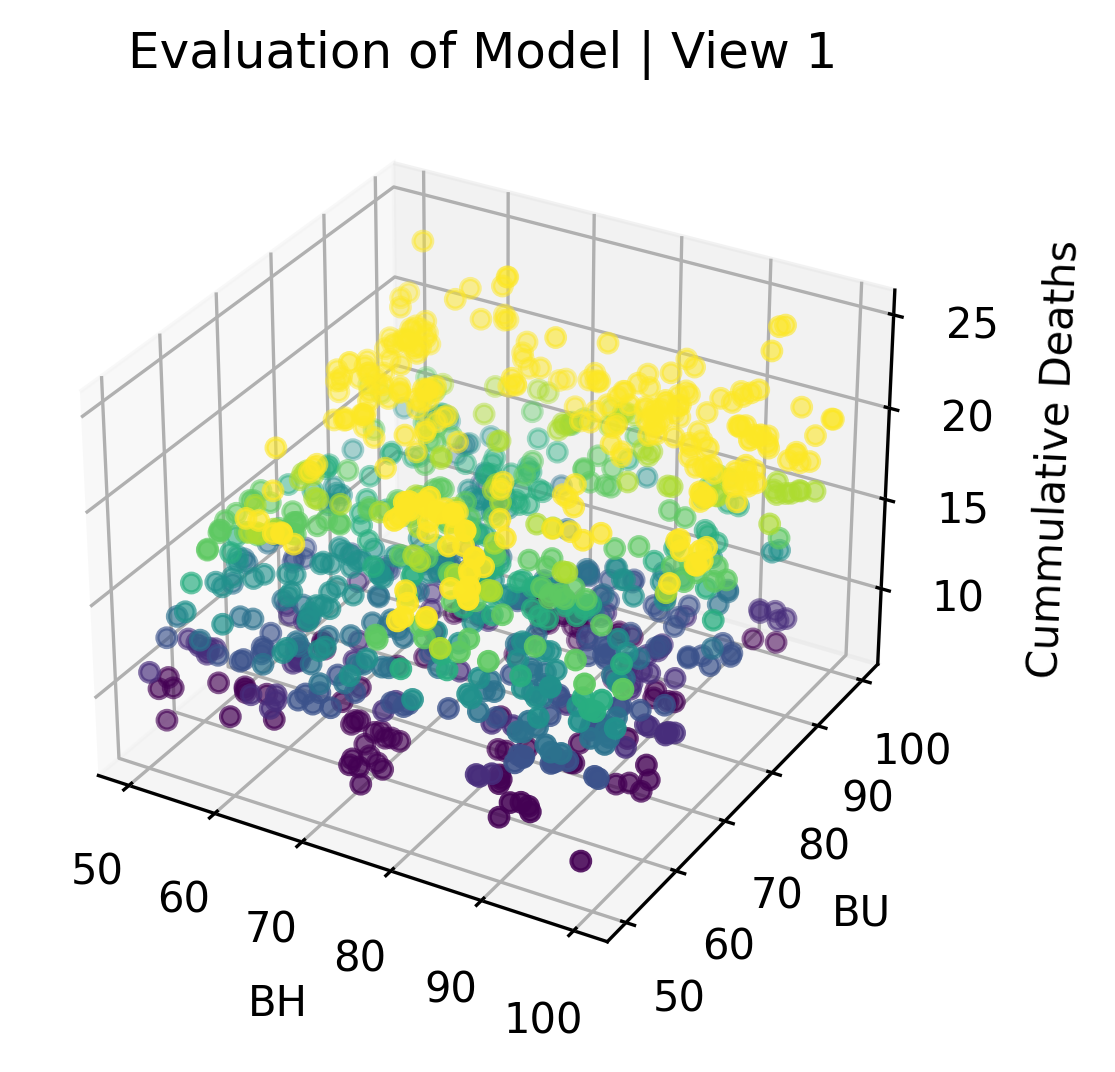
\includegraphics[width = .42\textwidth]{GT_Sim1}
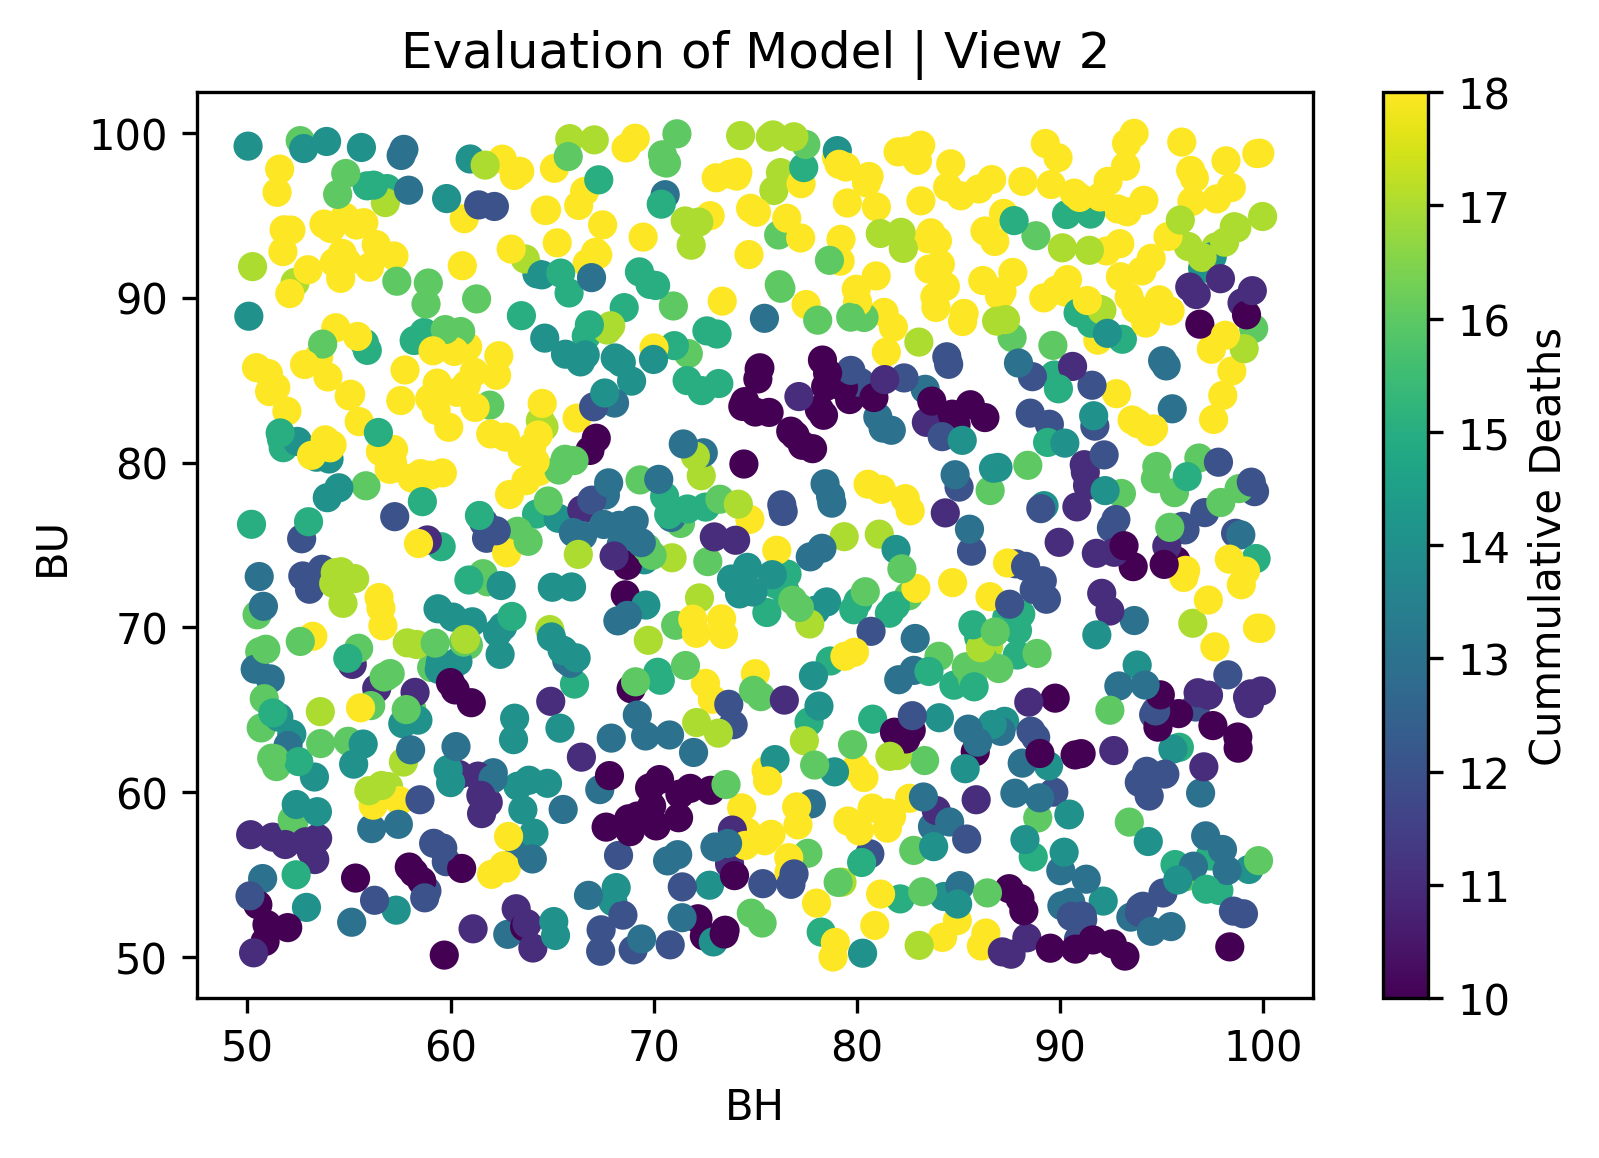
\includegraphics[width = .55\textwidth]{GT_Sim2}

\end{frame}


\begin{frame}
\frametitle{Problem 3 $|$ Task 3a | IDW Approach}

My Inverse Distance Weighted (IDW) attempt to metamodel the data is shown below. All the metamodeling methods are compared to the ``ground truth'' at the end of these slides. 


\vspace{.5em}
\centering
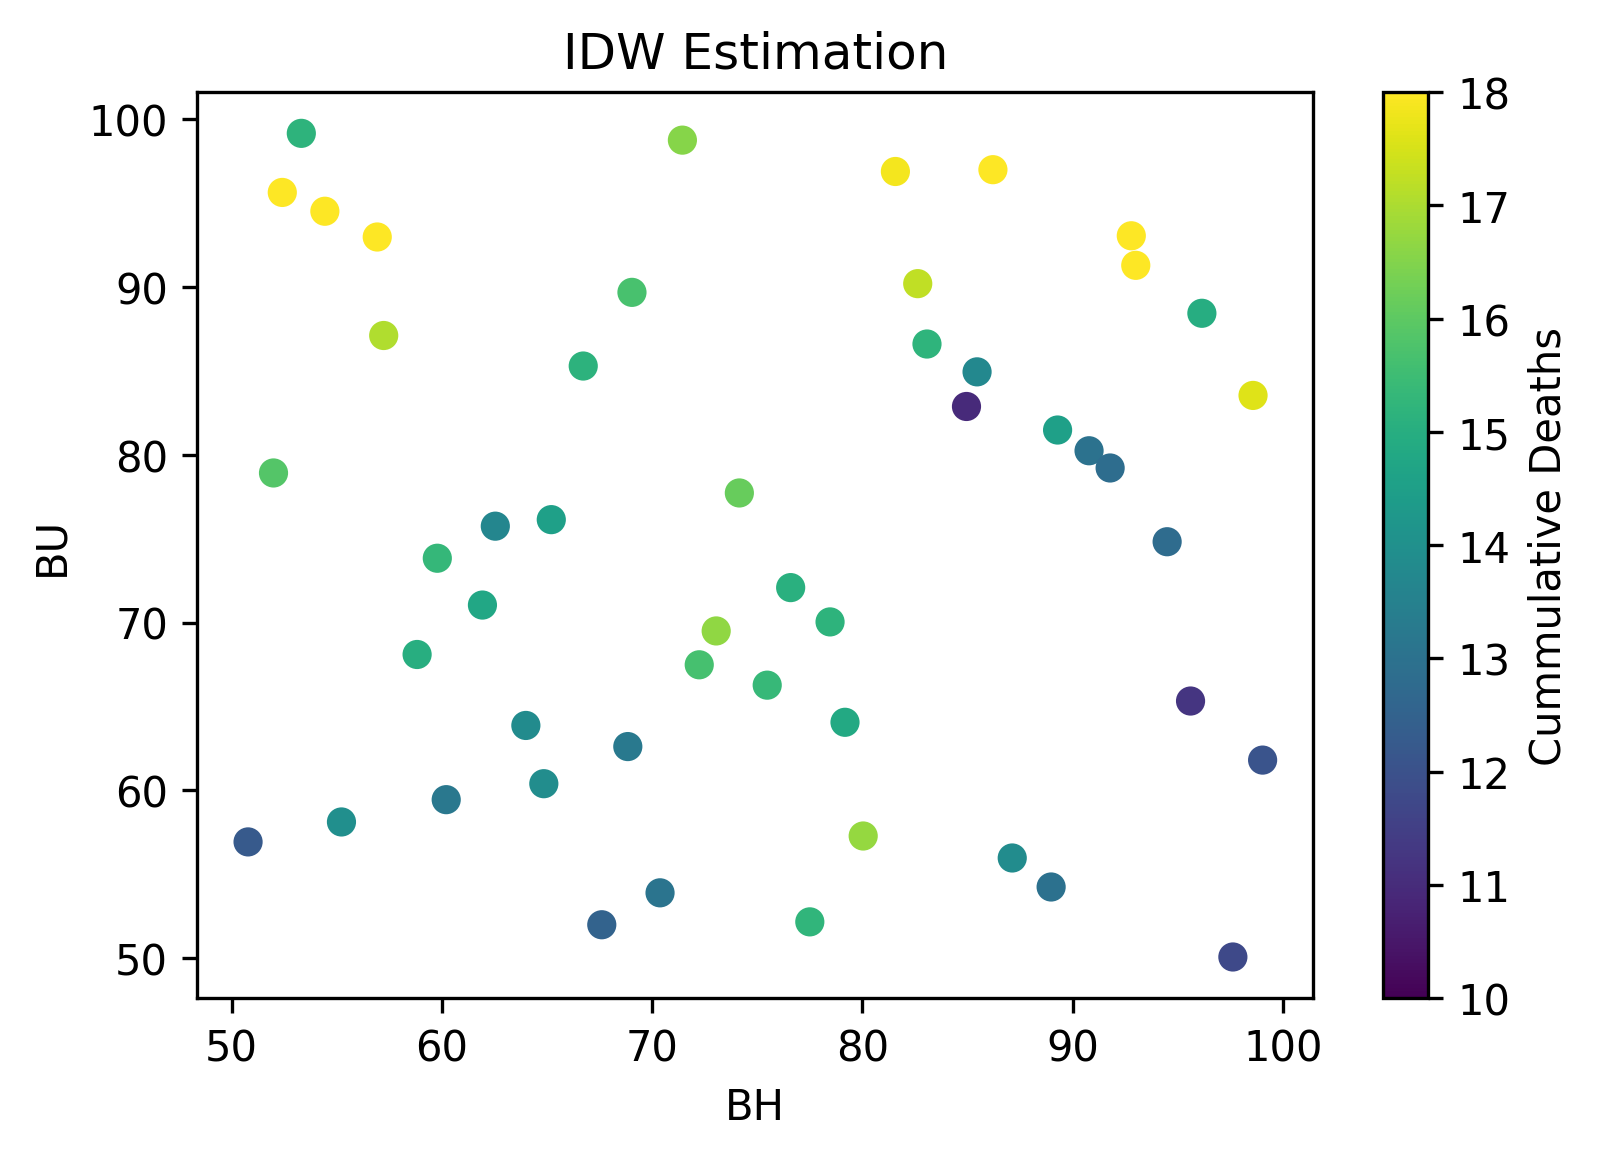
\includegraphics[width = .6\textwidth]{IDW}

\end{frame}


\begin{frame}
\frametitle{Problem 3 $|$ Task 3b | RBF Approach}

My Radial Basis Function (RBF) approach was as follows. I simulated this using a linear, cubic, and multiquadratic approach. I was not sure what was meant by combining cubic and linear approach...


\vspace{1em}

\centering
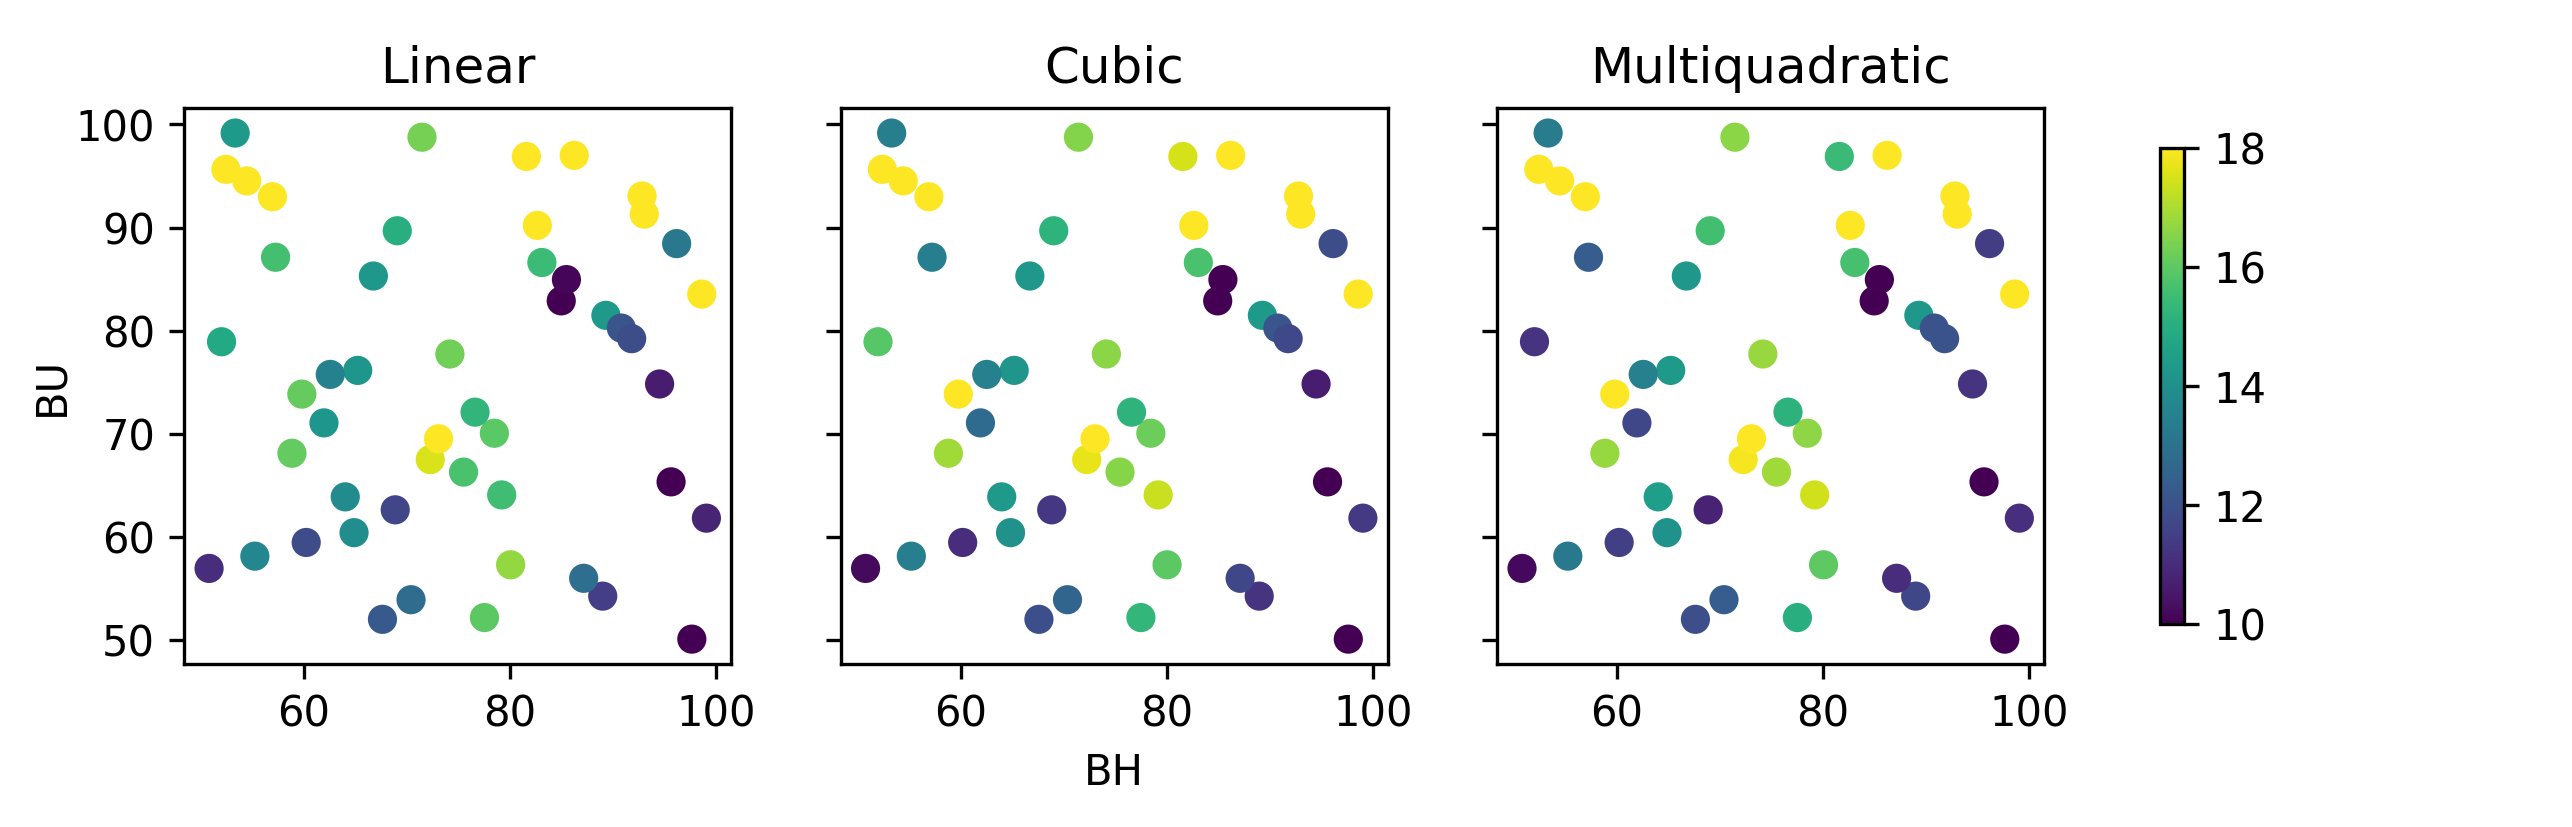
\includegraphics[width = .99\textwidth]{RBF}

\end{frame}

\begin{frame}
\frametitle{Problem 3 $|$ Task 3c/d | Neural Net and SVR Approaches}

Here are my ANN and Support Vector Regression (SVR). For the ANN approach, I allowed a maximum of 1000 iterations.

\vspace{1em}

\centering
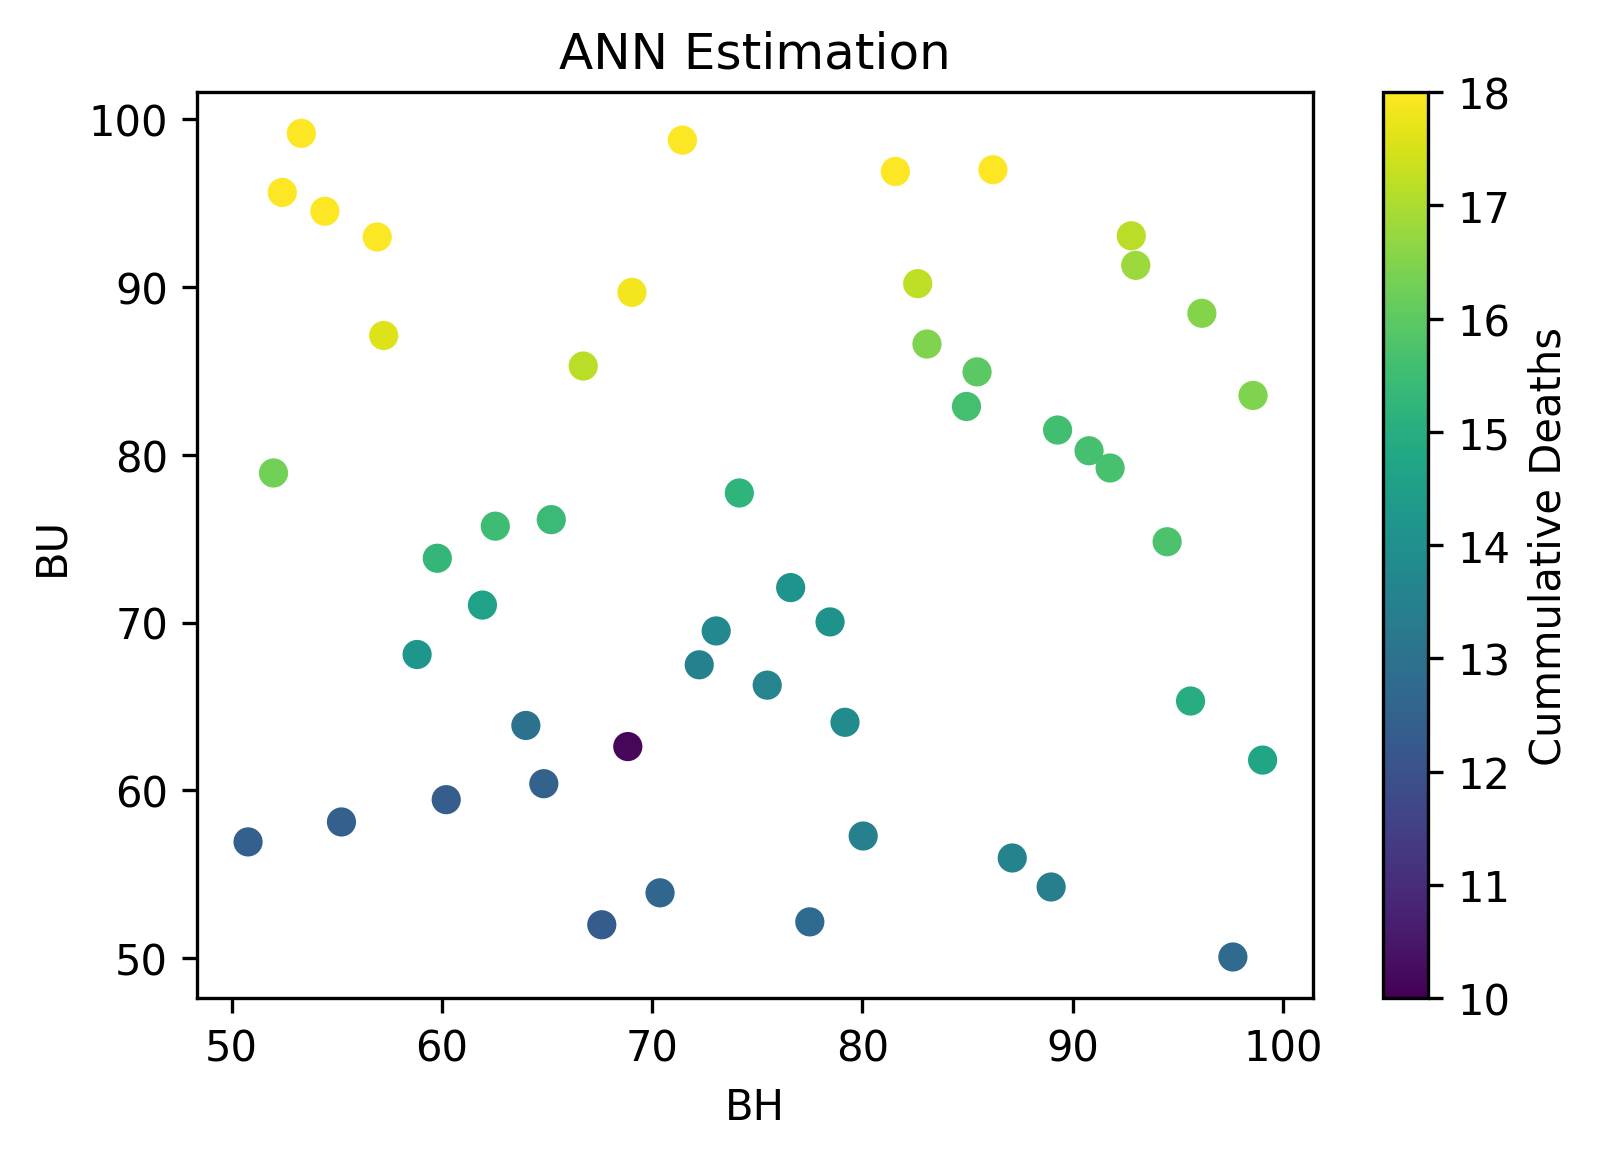
\includegraphics[width = .45\textwidth]{ANN}
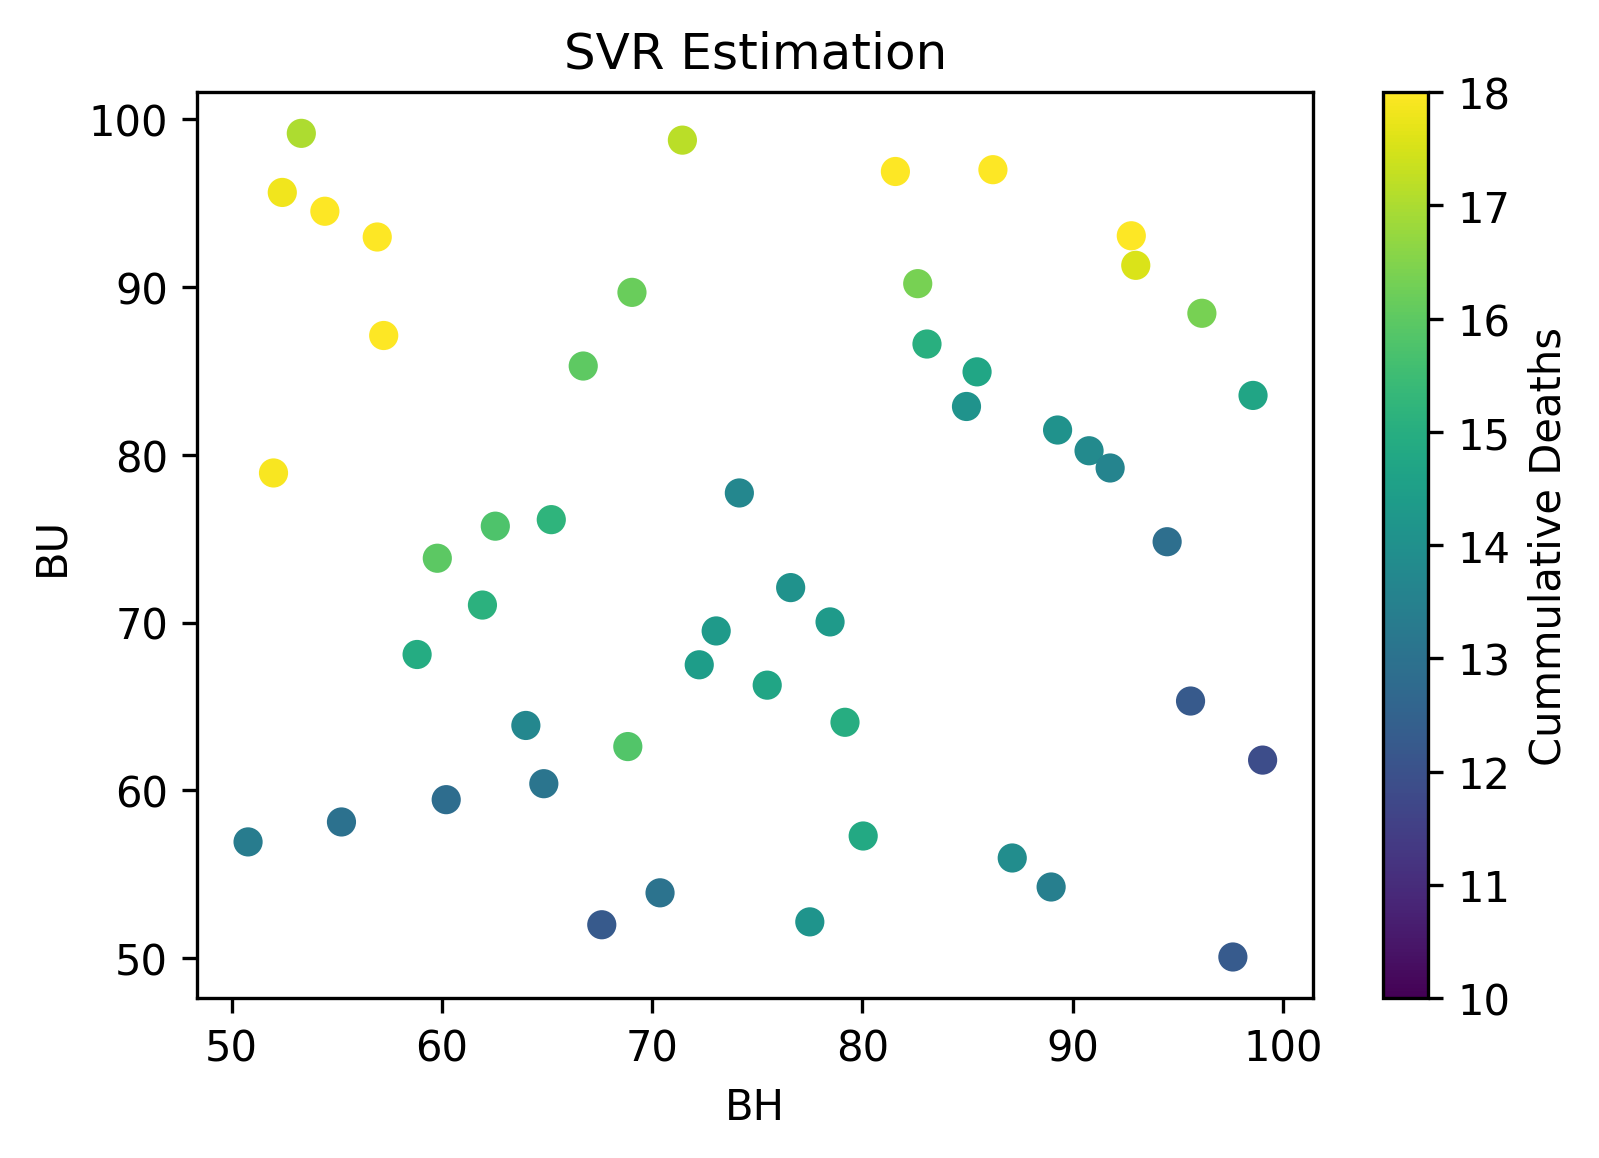
\includegraphics[width = .45\textwidth]{SVR}
\end{frame}


\begin{frame}
\frametitle{Problem 3 $|$ Comparisons to Ground Truth}

\footnotesize{To compare these metamodeling approaches to the ground truth, I used mean square error (MSE). It appears the RBF linear and IDW approaches resulted in the best representation of the model, with MSE $\approx$ 5. I am attaching my ipythonnotebook output to this slide deck in case there are any dependency-related issues to whomever may read this.}

\vspace{1em}

\centering
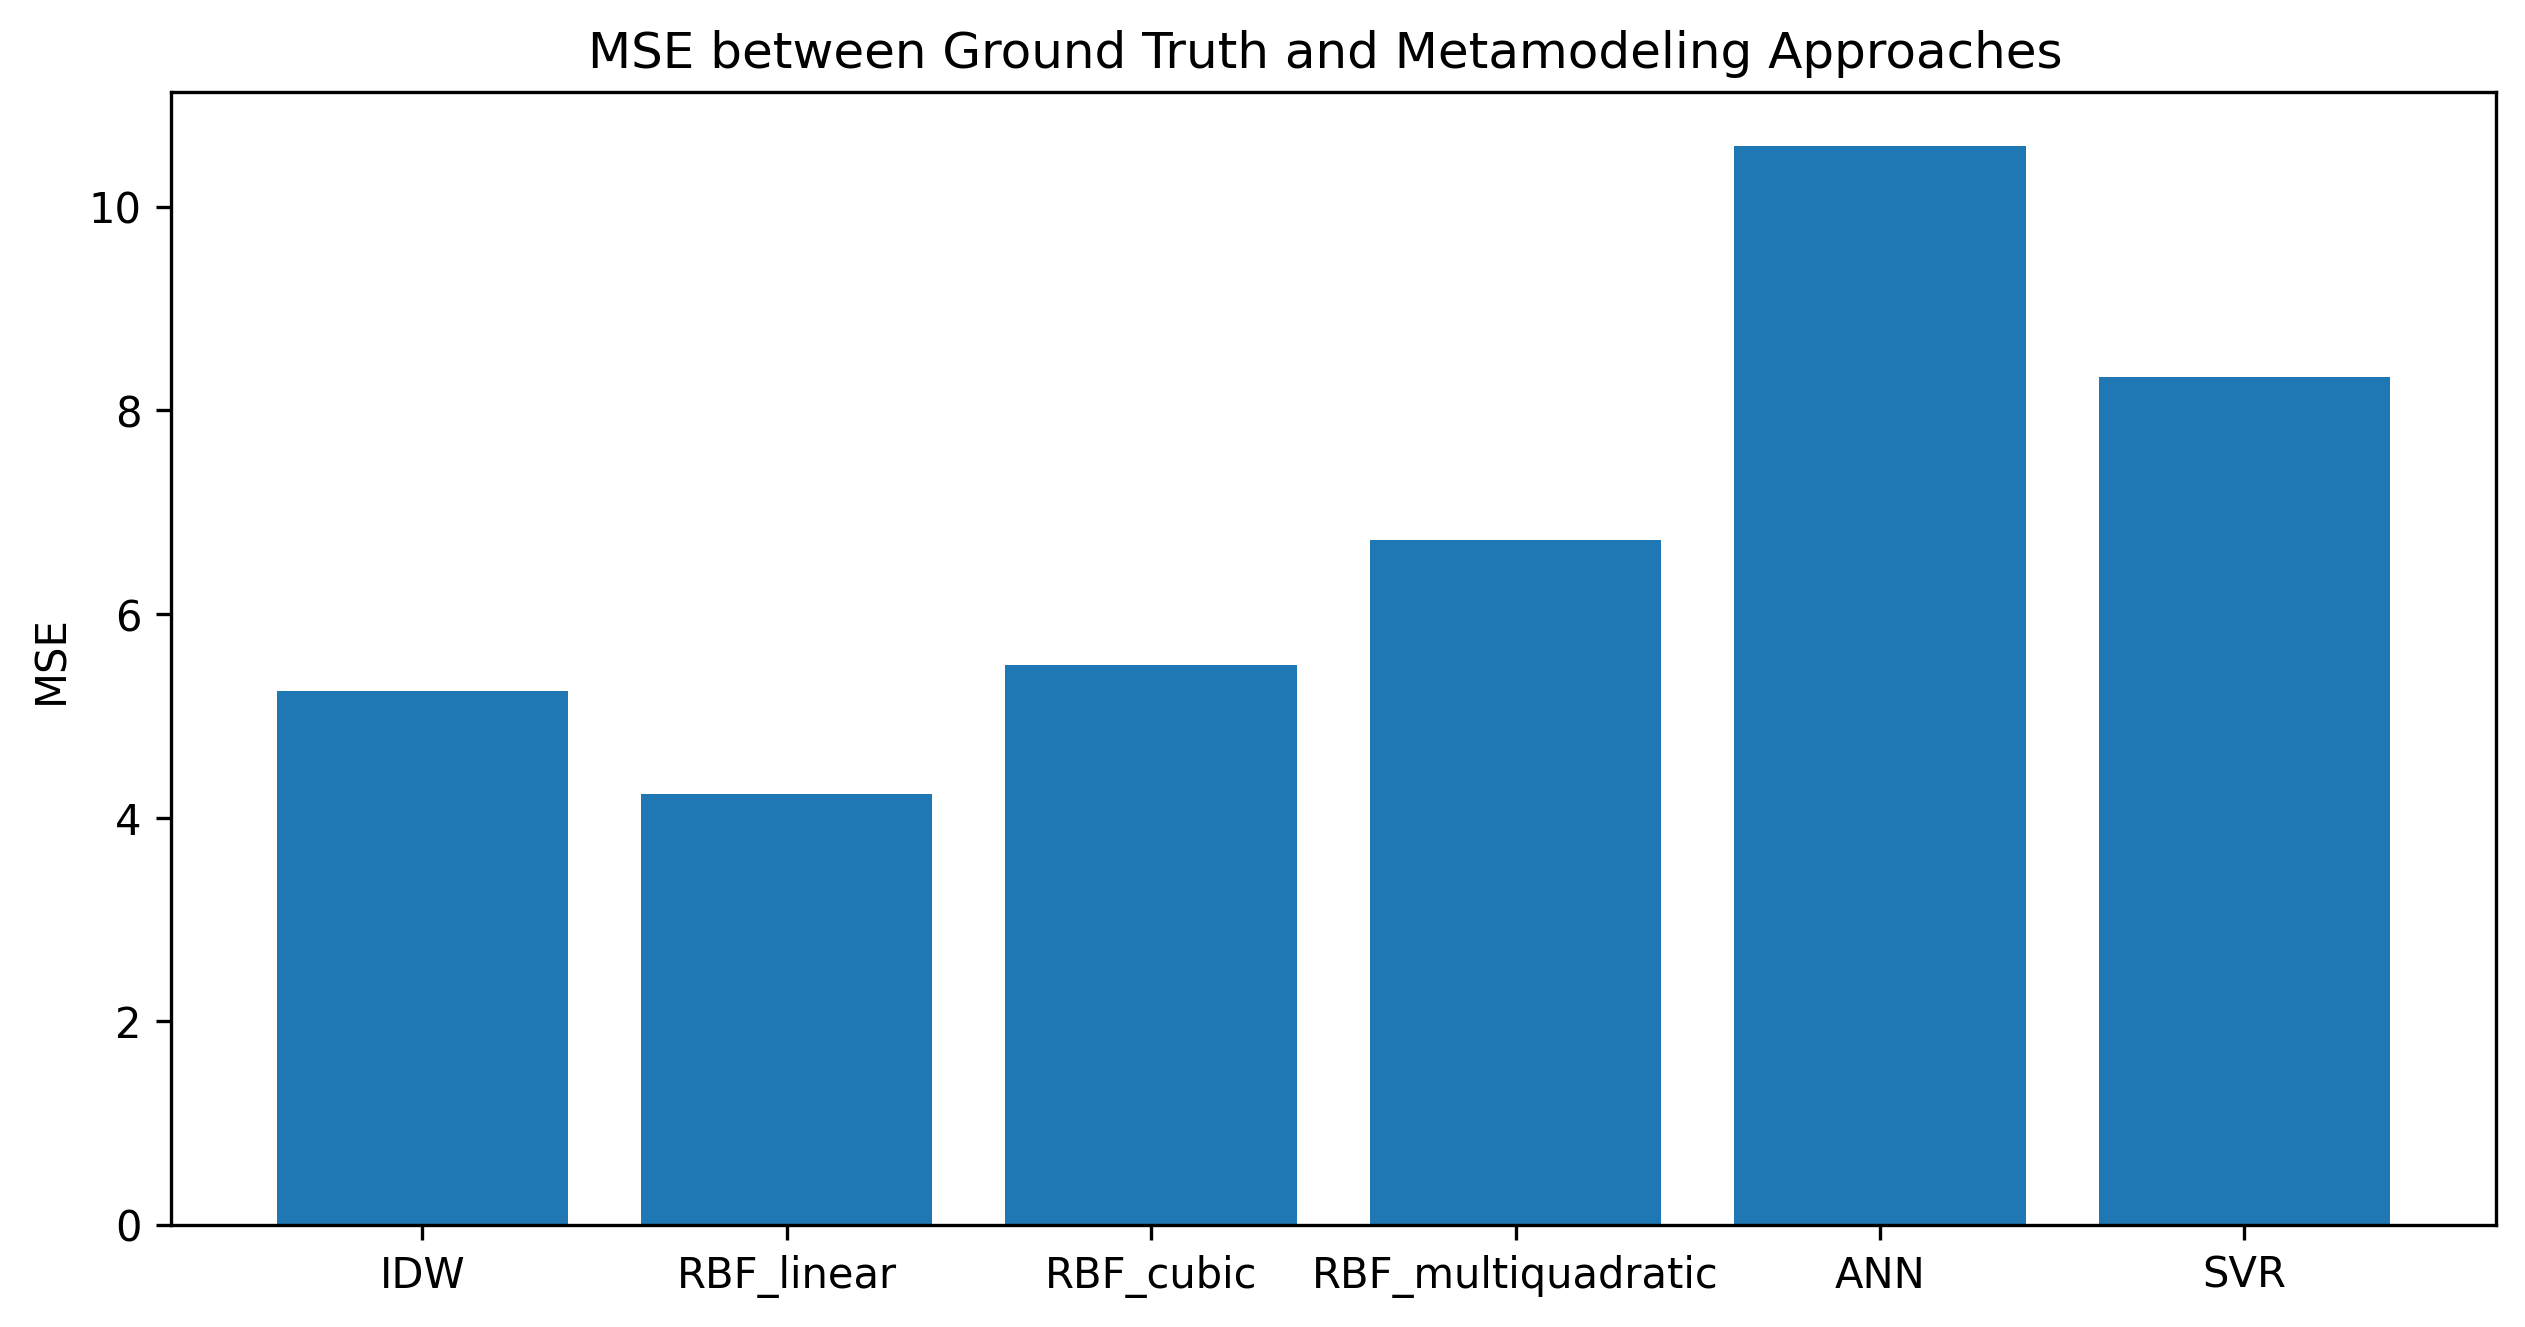
\includegraphics[width = .85\textwidth]{comparison}
\end{frame}

\end{document}